\documentclass[a4paper, 14 pt, titlepage]{extarticle}

\usepackage{grffile}
\usepackage{cmap}					% поиск в PDF
\usepackage[english,russian]{babel}	% локализация и переносы
\usepackage{indentfirst} 
\frenchspacing
\usepackage{setspace}
\usepackage{fontspec}      %% подготавливает загрузку шрифтов Open Type, True Type и др.
\defaultfontfeatures{Ligatures={TeX},Renderer=Basic}  %% свойства шрифтов по умолчанию
\setmainfont[Ligatures={TeX,Historic}]{Times New Roman} 
\setmonofont{Courier New}

\usepackage{amsmath,amsfonts,amssymb} 
\usepackage{amsthm}
\usepackage{mathtools}
\usepackage{icomma}

\renewcommand{\epsilon}{\ensuremath{\varepsilon}}
\renewcommand{\phi}{\ensuremath{\varphi}}
\renewcommand{\kappa}{\ensuremath{\varkappa}}
\renewcommand{\le}{\ensuremath{\leqslant}}
\renewcommand{\leq}{\ensuremath{\leqslant}}
\renewcommand{\ge}{\ensuremath{\geqslant}}
\renewcommand{\geq}{\ensuremath{\geqslant}}
\renewcommand{\emptyset}{\varnothing}

\usepackage{ragged2e}

\usepackage[unicode, pdfencoding=auto]{hyperref}
\usepackage[usenames,dvipsnames,svgnames,table,rgb]{xcolor}
\hypersetup{
            unicode=true,
            colorlinks=true,
            linkcolor=black,
            urlcolor=black,
            citecolor=black
           }

\usepackage{graphicx}
\graphicspath{{images/}}
\usepackage{wrapfig}
\usepackage{tikz}

\usepackage{listings}
\usepackage{color}

\lstset{
	basicstyle=\footnotesize\ttfamily,
	tabsize=4,
	columns=fixed,
	extendedchars=true,
	lineskip=-0.05\baselineskip,
	aboveskip=6pt,
	belowskip=6pt,
	breaklines,
	showstringspaces
}

\usepackage{cite}
\addto\captionsrussian{\renewcommand{\refname}{СПИСОК ИСПОЛЬЗОВАННЫХ ИСТОЧНИКОВ}}
\addto\captionsrussian{\renewcommand{\contentsname}{СОДЕРЖАНИЕ}}
\usepackage[titletoc]{appendix}
\addto\captionsrussian{\renewcommand{\appendixname}{Приложение}}
%\usepackage{tocloft}
%\usepackage{tocstyle}

\usepackage{array,tabularx,tabulary,booktabs, longtable, multirow}

\usepackage{etoolbox}
\usepackage{caption}
\captionsetup{labelsep=endash, font={singlespacing}, figurename=Рисунок }

\usepackage{lastpage}
\usepackage{fancyhdr} % Колонтитулы
 	\pagestyle{fancy}
 	\renewcommand{\headrulewidth}{0pt}  % Толщина линейки сверху
    \fancyfoot[R]{}
    \fancyfoot[C]{\thepage}
    \fancyhead[R]{}
    \fancyhead[L]{}
    
\setstretch{1.5}

\usepackage{extsizes}
\usepackage{geometry}
\geometry{top=2cm}
\geometry{bottom=2cm}
\geometry{left=3cm}
\geometry{right=1.5cm}

\usepackage{titlesec}

\renewcommand{\thesection}{\arabic{section}}
%\titleformat{\section}{\centering\normalsize \normalfont \bfseries }{\thesection}{1ex}{~\\\centering}[]
\titleformat{\section}{\centering\normalsize\normalfont\bfseries\uppercase}{\thesection.}{0.7ex}{}

\renewcommand{\thesubsection}{\thesection.\arabic{subsection}}
\titleformat{\subsection}{\normalsize\normalfont \bfseries}{\thesubsection.}{0.7ex}{}
\titlespacing\subsection{1.25cm}{1cm}{0pt}

\renewcommand{\thesubsubsection}{\thesubsection.\arabic{subsubsection}}
\titleformat{\subsubsection}{\normalsize\normalfont}{\thesubsubsection.}{0.7ex}{}
\titlespacing\subsubsection{1.25cm}{1cm}{0pt}

%\parindent=1.25cm
\setlength{\parindent}{1.25cm}

\newcommand{\startcode}{
    \footnotesize
    \singlespacing
}

\newcommand{\finishcode}{\setstretch{1.5}\normalsize}

\newenvironment{code}{\startcode}{\finishcode}

\newcommand{\printcaption}[1]{
    \normalsize
    {
    \captionsetup{justification=raggedright, singlelinecheck=off}
    \caption{#1}
    }
}




\newcommand{\subject}{Название дисциплины}
\newcommand{\labnumber}{1}
\newcommand{\teacher}{Петров~П.П.}
\newcommand{\theme}{Название темы}
\newcommand{\name}{Иванов~И.И.}

\begin{document}

\begin{titlepage}
   
   \begin{center}
       {\linespread{1.5}
        \textbf{
             МИНОБРНАУКИ РОССИИ\\
             САНКТ-ПЕТЕРБУРГСКИЙ
             ГОСУДАРСТВЕННЫЙ
             ЭЛЕКТРОТЕХНИЧЕСКИЙ
             УНИВЕРСИТЕТ\\ <<ЛЭТИ>> ИМ.~
             В.И.~УЛЬЯНОВА (ЛЕНИНА)\\
            Кафедра МО ЭВМ\\
            \vspace{7cm}
            ОТЧЁТ\\
            по учебной практике\\
            Тема: \theme\\
        }
        
        \vspace{4cm}
        
       
       
       \setlength{\extrarowheight}{4mm}
       \begin{tabulary}{\textwidth}{LCCCL}
            Студент гр. \groupnumber & \hspace{0.5cm} & \hspace{4.5cm} & \hspace{0.5cm} & \firstmember \\
            \cline{3-3}
            Студент гр. \groupnumber & \hspace{0.5cm} & \hspace{4.5cm} & \hspace{0.5cm} & \secondmember \\
            \cline{3-3}
            Студент гр. \groupnumber & \hspace{0.5cm} & \hspace{4.5cm} & \hspace{0.5cm} & \thirdmember \\
            \cline{3-3}
            Руководитель & \hspace{0.5cm} & \hspace{4.5cm} & \hspace{0.5cm} & \teacher \\
            \cline{3-3}
       \end{tabulary}
       \setlength{\extrarowheight}{0mm}
       
       \vfill
       
       Санкт-Петербург\\
       \the\year\\
       }
       
   \end{center}
   
  \end{titlepage}




\setcounter{page}{2}

\subsection*{Цель работы.}

\subsection*{Выполнение работы.}

\begin{figure}[h!]
	\centering
	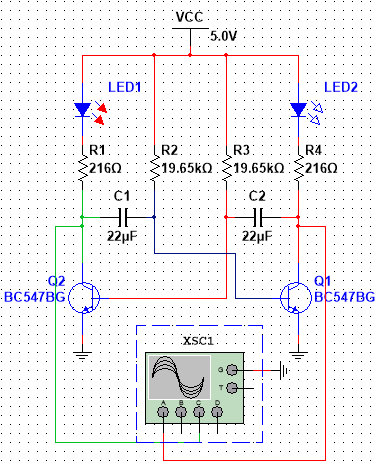
\includegraphics[width=0.7\linewidth]{images/image}
	\caption{Наименование иллюстрации}
	\label{fig:image}
\end{figure}


\subsection*{Тестирование.}

\subsection*{Вывод.}

\newpage
\section{Название приложения}

\end{document}
